% Chapter 3

\chapter{Methodology} % Main chapter title

\label{Chapter3} % For referencing the chapter elsewhere, use \ref{Chapter3}

%----------------------------------------------------------------------------------------

This chapter details the multi-model methodology for transforming unstructured biomedical text into a structured medical knowledge graph. The overall approach is a \textbf{pipeline} that sequentially performs entity recognition, entity linking, relationship extraction, and graph construction. By chaining specialized components, the system produces an \textbf{interpretable representation of medical concepts (e.g. drugs, diseases) and the relations among them}, enabling integration of context and supporting clinical insights. Key design decisions, data preprocessing steps, model configurations, and implementation optimizations are discussed in the following sections.

\section{System Architecture and Pipeline}

\subsection{Overall System Design}

The proposed system follows a modular pipeline architecture, where each stage transforms the biomedical text and feeds into the next stage. The architecture consists of the following major components and data flow:

\begin{figure}[h]
\centering
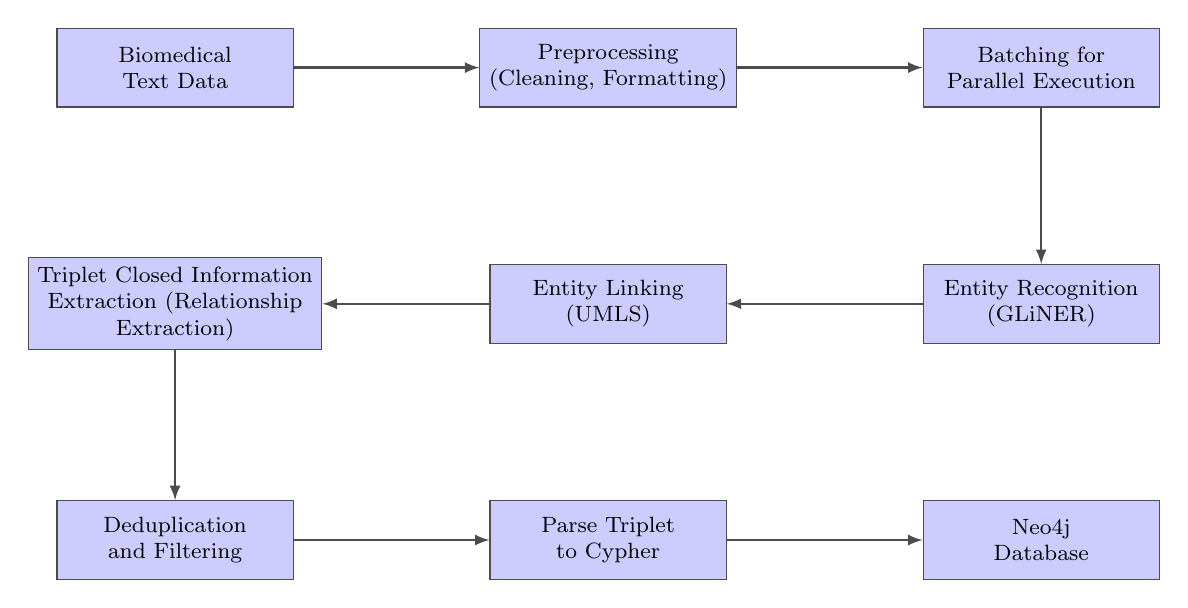
\begin{tikzpicture}[
    node distance=5.5cm,
    every node/.style={align=center},
    block/.style={rectangle, draw=black!70, fill=blue!20, minimum width=3cm, minimum height=1cm, font=\footnotesize},
    arrow/.style={->, >=latex, thick, draw=black!70}
]
    % Nodes - Following the specified order
    \node[block] (data) {Biomedical\\Text Data};
    \node[block, right of=data] (preprocess) {Preprocessing\\(Cleaning, Formatting)};
    \node[block, right of=preprocess] (batching) {Batching for\\Parallel Execution};
    \node[block, below of=batching, node distance=3cm] (ner) {Entity Recognition\\(GLiNER)};
    \node[block, left of=ner] (linking) {Entity Linking\\(UMLS)};
    \node[block, left of=linking] (relation) {Triplet Closed Information\\Extraction (Relationship\\Extraction)};
    \node[block, below of=relation, node distance=3cm] (dedup) {Deduplication\\and Filtering};
    \node[block, right of=dedup] (cypher) {Parse Triplet\\to Cypher};
    \node[block, right of=cypher] (save) {Neo4j\\Database};
    
    % Arrows - Following the specified flow
    \draw[arrow] (data) -- (preprocess);
    \draw[arrow] (preprocess) -- (batching);
    \draw[arrow] (batching) -- (ner);
    \draw[arrow] (ner) -- (linking);
    \draw[arrow] (linking) -- (relation);
    \draw[arrow] (relation) -- (dedup);
    \draw[arrow] (dedup) -- (cypher);
    \draw[arrow] (cypher) -- (save);

\end{tikzpicture}
\caption{System architecture pipeline showing the transformation of biomedical text into a knowledge graph}
\label{fig:system-architecture}
\end{figure}

\begin{enumerate}
\item \textbf{Input and Preprocessing:} Raw biomedical text (free-text) is first collected and preprocessed (cleaning, formatting) to ensure consistent input for NLP tasks.
\item \textbf{Entity Recognition:} A biomedical Named Entity Recognition (NER) model identifies spans of text corresponding to biomedical concepts (e.g. genes, diseases, chemical compounds, variants, species). We employ the GLiNER model for this step (see Section~\ref{sec:gliner}).
\item \textbf{Entity Linking:} Detected entity mentions are normalized and linked to a canonical identifier in a medical knowledge base. We use SciSpacy's UMLS linker to map each mention to a UMLS Concept Unique Identifier (CUI), providing standardized meanings (Section~\ref{sec:entitylinking}).
\item \textbf{Relationship Extraction:} A large language model (LLM) processes the linked entity list and full text to extract relationships between the medical entities. The model outputs structured triple relationship assertions (Section~\ref{sec:relationextraction}).
\item \textbf{Knowledge Graph Construction:} The extracted entities and relationships are inserted into a Neo4j graph database. Nodes represent medical concepts (annotated with UMLS CUIs and types) and edges represent the relationships between concepts. Cypher queries are generated to create or merge these graph elements (Section~\ref{sec:graphconstruction}).
\item \textbf{Post-processing \& Optimization:} Throughout the pipeline, confidence filters, validation checks, and parallelization are applied to ensure quality and efficiency (Section~\ref{sec:optimization}).
\end{enumerate}

Each component addresses a specific task, and their integration yields a coherent end-to-end system. This design allows independent optimization of each module and the ability to swap models if needed. The multi-step \textbf{``recognition→linking→relation extraction→graph loading''} strategy aligns with recommended knowledge graph construction practices, ensuring that unstructured text is incrementally converted into a structured, interoperable knowledge graph.

\subsection{Component Integration Flow}

The flow of data between components is carefully orchestrated to preserve context and accuracy. The pipeline is implemented as a \textit{sequential workflow} where each module consumes the outputs of previous steps:

\begin{itemize}
\item The \textbf{Preprocessing} stage standardizes the input. This may include lowercasing (if required by the NER model), removing extraneous whitespace or headers, and ensuring patient-identifying information is excluded for privacy (see Section~\ref{sec:datapreprocessing}).
\item The \textbf{NER component} (GLiNER) is applied next on the cleaned text. It produces a set of entity mentions (text spans) each with an entity type (e.g. \textit{Condition}, \textit{Drug}, \textit{Test}). These mentions are passed forward as Python objects (e.g. spaCy \texttt{Span} objects) attached to the document representation.
\item The \textbf{Entity Linking} module (SciSpacy's \texttt{EntityLinker}) takes each NER-detected span and searches for candidate concepts in the UMLS knowledge base. Because this linker is integrated as a spaCy pipeline component, it can enrich the detected \texttt{Span} with a list of candidate CUIs and similarity scores (available via \texttt{Span.\_.kb\_ents}). We configure the linker to resolve abbreviations and to attach the top-ranked CUI for each mention above a confidence threshold (details in Section~\ref{sec:confidence}). The result is that each entity mention from NER is now linked to a unique medical concept ID or marked as \textit{unlinkable} if no high-confidence match is found.
\item For \textbf{Relationship Extraction}, the entire biomedical document along with the recognized entities is provided to the LLM. In practice, we construct a prompt that includes the text and possibly the list of identified entities, asking the model to output relationships (e.g. cause/effect, treatment, associations) among those entities. The integration is such that the model's output can be traced back to the original entities by name or CUI. This output is captured as structured relation triples.
\item Finally, the \textbf{Graph Construction} module translates the entities and relations into Cypher queries. The integration here uses the results of previous steps (entity CUIs, names, types, and relation types) to form \texttt{MERGE} statements. For example, if ``C0011849'' (Diabetes mellitus) and ``C0027796'' (Neuropathy) are two CUIs with a \textit{causes} relationship, the pipeline will generate a Cypher command to \texttt{MERGE} nodes for each (with labels/types) and a \texttt{[:CAUSES]} relationship between them. These queries are executed on the Neo4j database to update the knowledge graph.
\end{itemize}

Throughout this flow, \textbf{state is maintained} so that each mention's context is known. For instance, if an LLM-produced relationship mentions an entity not recognized by NER, we detect that during parsing and handle it (either by discarding that relation or attempting to link the new entity, as discussed in Section~\ref{sec:outputparsing}). This ensures consistency: only vetted entities make it into the graph. The sequential integration also means errors can propagate (e.g. a linking error could affect relation extraction), so each component is tuned to maximize precision, and wherever possible, the pipeline includes verification steps (for example, ensuring that relation arguments have valid CUIs). The design balances modularity with tight integration, creating a robust system to extract structured knowledge from biomedical text.

\section{Data and Preprocessing}
\label{sec:datapreprocessing}

\subsection{Biomedical Literature Dataset and Preparation}

Our dataset consists of biomedical literature from the \textbf{BioRED} dataset, a comprehensive corpus for biomedical relation extraction. BioRED contains manually annotated PubMed abstracts with multiple entity types (gene/gene products, diseases/phenotypic features, chemical entities, variants, species, and cell lines) and their relationships. The dataset provides over 6,000 annotated documents with more than 30,000 entity mentions and 6,000 relationship annotations across eight relation types including Association, Positive\_Correlation, Negative\_Correlation, Bind, Comparison, Cotreatment, Drug\_Interaction, and Conversion. These abstracts represent diverse biomedical research areas and contain domain-specific terminology, complex medical concepts, and scientific relationships. The dataset is particularly valuable for developing and evaluating biomedical NLP systems as it captures the complexity of scientific literature while providing gold-standard annotations. Before applying the NLP pipeline, we perform several preprocessing steps to prepare this data:

\begin{itemize}
\item \textbf{PubTator Format Parsing:} The BioRED dataset is provided in PubTator format, a standardized format for biomedical text annotations. Each document contains a PubMed ID (PMID), title, abstract, entity annotations with character offsets, and relation annotations linking entity IDs. We parse this format to extract the text content and gold-standard annotations for evaluation purposes.
\item \textbf{Text Reconstruction:} We combine the title and abstract sections to form complete documents for processing. The character offsets from entity annotations are preserved to enable precise evaluation against our pipeline's predictions. We ensure proper spacing between title and abstract to maintain text coherence.
\item \textbf{Entity Type Mapping:} BioRED uses specific entity type labels (GeneOrGeneProduct, DiseaseOrPhenotypicFeature, ChemicalEntity, etc.) which we map to our pipeline's entity categories. This mapping ensures compatibility between the dataset's annotation schema and our NER model's expected input types.
\item \textbf{Relation Type Standardization:} The dataset includes eight relation types with specific biomedical meanings. We preserve these relation types for evaluation while ensuring they align with our relationship extraction model's output format. Relations are provided as entity ID pairs, which we resolve to actual text mentions using the entity annotations.
\end{itemize}

After preprocessing, the biomedical abstracts are properly formatted and their annotations are structured for evaluation. This careful preparation facilitates accurate assessment of our pipeline's performance against gold-standard annotations. The preprocessing ensures that entity boundaries are preserved, relation pairs are correctly mapped, and the text maintains its scientific accuracy. These steps address the \textbf{``garbage in, garbage out''} concern - proper data preparation is essential for meaningful evaluation and reliable knowledge extraction from biomedical literature.

\section{Entity Recognition and Linking}

\subsection{GLiNER Model for Medical Entity Recognition}
\label{sec:gliner}

For identifying medical entities in text, we utilize the \textbf{GLiNER} model – a \textit{Generalist and Lightweight Named Entity Recognition} framework adapted for biomedical data. Traditional medical NER is challenging due to vast evolving healthcare vocabulary and limited labeled training data. GLiNER offers \textbf{open-domain, zero-shot NER} using \textit{natural language descriptors} rather than fixed entity taxonomies. We can prompt GLiNER with definitions like medical condition'' or drug name,'' and it identifies corresponding text spans.

GLiNER-BioMed leverages large language models for annotation, then distills knowledge into smaller, efficient NER models. Developers generated synthetic training data using LLMs, then trained GLiNER models on this data. The result achieves state-of-the-art biomedical NER performance with 6\% F1-score improvement over previous systems in zero-shot scenarios, statistically significant at p < 0.001 \parencite{Stenetorp2024}.

In our pipeline, we chose GLiNER for its generalization ability, configuring it with \textbf{medical entity type prompts}: \textit{Problem/Condition}, \textit{Treatment/Drug}, \textit{Test/Procedure}, and others as needed. GLiNER can tag entities without dataset-specific retraining. For \textit{The patient was started on metformin for diabetes mellitus''}, GLiNER identifies \textbf{metformin''} as Drug and \textbf{``diabetes mellitus''} as Condition based on prompt understanding.

GLiNER's \textbf{lightweight architecture} is smaller and faster than full LLMs, suitable for scanning long documents. It effectively \textit{distills} larger models' linguistic knowledge into specialized NER tasks, running efficiently on available compute (Apple Silicon CPU/GPU) with reasonable speed crucial for biomedical text processing.

\subsection{UMLS Entity Linking with SciSpacy}
\label{sec:entitylinking}

Once entities are recognized, we perform \textbf{entity linking} to anchor mentions to standardized medical ontology using SciSpacy's UMLS \textbf{EntityLinker} for biomedical normalization. SciSpacy provides spaCy models tailored to scientific/clinical text \parencite{Neumann2019}, with entity linker containing a built-in knowledge base from the \textbf{Unified Medical Language System (UMLS)} Metathesaurus integrating millions of biomedical concepts.

SciSpacy's linking algorithm uses \textbf{string similarity} with \textit{character n-grams}, representing entity mentions as bag-of-character-trigrams with \textbf{TF-IDF weighted vectors}. Every UMLS concept name is indexed by character trigrams, enabling approximate nearest neighbor search for most similar concepts. This finds overlapping substrings - robust for biomedical text with lexical variants, like cardiac infarction'' matching \textit{Myocardial Infarction''} through trigram overlap.

We configured SciSpacy with \texttt{\detokenize{linker_name="umls"}} and \texttt{\detokenize{resolve_abbreviations=True}} to expand short forms before linking. The UMLS knowledge base includes primary vocabularies totaling roughly 3 million concepts. We kept the default \textbf{similarity threshold} of 0.7, meaning linkers only assign concepts when cosine similarity between TF-IDF trigram vectors is $\geq 0.7$, filtering tenuous matches and improving precision.

During linking, SciSpacy produces candidate concept IDs with similarity scores for each entity. We select top-ranked candidates exceeding the threshold. For metformin,'' the linker returns (CUI: C0025598, Metformin'', score 0.98), providing \textit{canonical representation} with UMLS Concept Unique Identifiers and standardized names, definitions, and semantic types.

Linking to UMLS creates \textbf{interoperable knowledge graphs}. Grounding entities to UMLS CUIs aligns nodes with established ontology, facilitating healthcare data integration and hierarchical queries. It consolidates synonyms - heart attack'' and myocardial infarction'' link to the same CUI, creating single graph nodes and avoiding duplication \parencite{UMLS2024}.

\subsection{Confidence Scoring and Abbreviation Detection}
\label{sec:confidence}

In this stage, we refine the outputs of NER and linking by incorporating confidence measures and handling abbreviations explicitly:

\begin{itemize}
\item \textbf{Confidence Scoring:} Both NER and linker provide internal scores. After entity linking, we use SciSpacy's \textbf{similarity score} as confidence proxy. Poor matches (0.4 similarity) may be dropped, while high scores (close to 1.0) indicate confident matches. We examine score distributions - if best match is 0.72 and second is 0.71, that's ambiguous; if best is 0.85 and second is 0.60, that's clear-cut. We set thresholds: below 0.7 marks entities as "Unlinked," above 0.9 accepts outright, and 0.7-0.9 accepts with lower confidence flags. This approach maintains knowledge graph quality by minimizing spurious nodes/edges.

\item \textbf{Abbreviation Detection:} Biomedical literature contains numerous abbreviations and acronyms requiring resolution for correct linking. We integrate SciSpacy's \textbf{AbbreviationDetector} implementing Schwartz \& Hearst algorithm \parencite{Schwartz2003}, scanning for patterns like ``Full Form (Abbr).'' For \textit{``tumor necrosis factor alpha (TNF-$\alpha$)''}, it detects \textbf{``TNF-$\alpha$''} abbreviates \textbf{``tumor necrosis factor alpha.''} With \texttt{resolve\_abbreviations=True}, the EntityLinker uses long forms for UMLS matching, yielding correct high-confidence links. This particularly helps with common biomedical abbreviations like ``IL'' (interleukin) by using local context for expansion.
\end{itemize}

By applying confidence scoring and abbreviation resolution, we \textbf{improve the precision and recall} of the entity linking process. High-confidence links and fully expanded terms result in more correct nodes in the graph, and fewer missed entities. These measures also reduce noise for the next stage: the relationship extraction model will receive text where abbreviations are already expanded (in the \texttt{Doc} object's context) and where uncertain entities can be treated cautiously. Overall, this step solidifies the foundation of the knowledge graph by ensuring that we have \textit{trusted, well-defined entities} to work with.

\section{Relationship Extraction}
\label{sec:relationextraction}

\subsection{Model Selection and Prompt Engineering}

Extracting relationships from biomedical text involves understanding semantic connections between medical entities. We approach this with \textbf{Large Language Models (LLMs)} that interpret text meaning and generate relational triples. We consider two LLMs: \textbf{Gemma} (general-purpose model) and \textbf{MedGemma} (specialized variant fine-tuned for medical domains). MedGemma, developed by Google DeepMind in 2025, demonstrates advanced medical understanding and clinical reasoning capabilities, building on Gemma's strengths with domain-specific training \parencite{MedGemma2025,Gemma2025}.

Given accurate relation extraction's critical nature, we experiment with both models. MedGemma (4B variant) is expected to excel at medical relationships (drug-disease interactions, symptom-disease associations), while Gemma provides a baseline for non-medical-tuned performance. The pipeline is \textit{model-agnostic}, accommodating any LLM accepting prompts and returning text.

We use a \textbf{prompt-based approach} (in-context learning) rather than fine-tuning to leverage models directly. Prompts are carefully engineered for structured output, following best practices that clearly define tasks, provide examples, and indicate desired formats \parencite{Reynolds2021}.

\begin{itemize}
\item A brief task description: e.g., \textit{``Extract all clinically relevant relationships between medical concepts in the following text.''}
\item A format instruction: e.g., \textit{``Provide the relationships as a list of triples (Subject, Relation, Object) using the exact entity names from the text.''} We explicitly ask for the model to use the entities as mentioned, to ease alignment with CUIs.
\item Optionally, a few-shot example: for instance, showing the model an example sentence and the extracted triple from it. We might include one or two demonstration pairs if it improves performance, although with very large models often a clear instruction suffices.
\item The context text: the actual biomedical document or a segment of it, possibly truncated to stay within token limits of the model.
\end{itemize}

An example prompt might be:

\begin{verbatim}
Extract all relationships between medical entities in the text. 
Use the format (Entity1, Relation, Entity2).
Text: "The patient's diabetes caused peripheral neuropathy and 
he was prescribed gabapentin for pain management."
Relationships:
1. (diabetes, causes, peripheral neuropathy)
2. (gabapentin, treats, pain)
\end{verbatim}

In this prompt, we provided a made-up example demonstrating the expected output format. The actual note's text would follow after ``Text:'' and we would expect the model's completion to list similar triples.

We also incorporate prompt elements to handle nuances: e.g., instruct the model to ignore trivial relations or to only output relations that are explicitly or implicitly stated (to avoid hallucination). We emphasize that the output should not include any entity not found in the text. This is important because LLMs have a tendency to infer or hallucinate facts; by explicitly saying \textit{``use only entities from the text''}, we reduce the chance the model introduces an unrelated concept.

To summarize, our prompt engineering strategy focuses on clarity, examples, and format enforcement. We aim to push the model to behave almost like a rule-based extractor but backed by its deep understanding of language. This harnesses the best of both worlds: the model's intelligence and a deterministic output scheme. We will quantitatively compare the two chosen models' outputs later, but here it's worth noting that using an LLM for relation extraction aligns with the latest research trends in knowledge graph construction. Large foundation models have been successfully used to perform relation extraction without extensive task-specific training, by virtue of their pre-trained knowledge and language understanding \parencite{Singhal2022}. Our methodology capitalizes on this capability by employing prompt-based LLM queries to extract rich relational information from text that simpler models or rule-based systems might miss.

\subsection{Output Parsing and Validation}
\label{sec:outputparsing}

After the LLM produces candidate relationships in text form, we need to parse these outputs and validate them before integration into the knowledge graph. This step is critical for maintaining accuracy and consistency, as the raw model output may contain noise or require interpretation.

\begin{itemize}
\item \textbf{Output Parsing:} Given structured output instructions, the parser interprets the format line by line with triples like \texttt{(Entity1, relation, Entity2)}. We implement regex or string splitting to extract triple components. From \texttt{(diabetes, causes, peripheral neuropathy)}'', the parser strips parentheses and splits by comma, yielding subject = diabetes'', relation = causes'', object = peripheral neuropathy''. We trim whitespace and ensure text matches the original note.

\item \textbf{Entity Matching:} We cross-match extracted entity text with NER-recognized entities. Each Entity1 and Entity2 should correspond to NER-identified mentions. For minor variations (model outputs diabetes'' but text had diabetes mellitus''), we match by substring or linked CUI since both share concepts. For entities entirely absent from text (likely hallucinations), we \textbf{discard that triple}. This post-hoc validation filters extraneous tokens/entities \parencite{Ji2023}.

\item \textbf{Relation Validation:} We validate relation parts, checking for reasonable expressions (verbs or short phrases) like causes,'' treats,'' ``indicates.'' We flag lengthy or dubious relation phrases and ensure relations aren't empty or identical to entities. Malformed outputs like \texttt{(X, X, Y)} are removed as nonsensical.

\item \textbf{Duplication and Uniqueness:} The parser handles duplicates when LLMs list relationships twice or express them similarly. We canonicalize triples (sorting/lowercasing relation phrases) and use sets for uniqueness. Most relations are directed (cause vs caused-by), so we treat \texttt{(diabetes, causes, neuropathy)} as distinct from \texttt{(neuropathy, causes, diabetes)}.

\item \textbf{Confidence and Post-Filtering:} Each triple inherits confidence estimated from model reliability and keyword presence. Relations directly from text (``caused'') have high confidence; inferred relations have lower confidence. MedGemma tends to stick closer to text while general models infer more, so we weight MedGemma triples slightly higher. We insert triples above basic confidence thresholds but tag questionable ones for potential analysis exclusion.
\end{itemize}

As a result of parsing and validation, we obtain a \textbf{clean set of (Subject, Relation, Object)} triples, each linked to UMLS concept IDs via the subject and object. For example, ``(diabetes mellitus, causes, peripheral neuropathy)'' becomes (CUI C0011849, \textit{causes}, CUI C0031117) after we replace the text with the corresponding CUIs from the earlier linking stage. These are now ready to be ingested into the knowledge graph. The validation steps, while reducing quantity slightly, ensure that the \textit{quality of relationships is high} – only those supported by the text and recognized entities are kept. This mitigates the risk of hallucinations or errors from the LLM contaminating the knowledge base. By designing the prompt and parser in tandem, we effectively constrain the LLM's output and then double-check it, achieving a balance between \textbf{completeness and accuracy} in relationship extraction.

\section{Knowledge Graph Construction}
\label{sec:graphconstruction}

\subsection{Graph Schema Design}

With a list of extracted entities (linked to UMLS) and relations, we define a schema for how these should be represented in the knowledge graph. The schema outlines what node types and relationship types exist, and what properties they carry, ensuring the graph is both expressive and normalized.

\begin{itemize}
\item \textbf{Node Types and Properties:} In our design, each \textbf{medical entity} becomes a node in the graph. Rather than having dozens of node categories for each fine-grained entity type, we opt for a unified node label, say \textbf{\texttt{:MedicalEntity}}, with properties to encode its attributes. Every node has at least:

  \begin{itemize}
  \item \textbf{\texttt{cui}}: the UMLS Concept Unique Identifier (as a string). This is the primary key for the node; we assume one node per unique CUI. Using CUI ensures that if the same concept appears in multiple notes, they map to the same node.
  \item \textbf{\texttt{name}}: a canonical name for the concept. We use the preferred name from UMLS for that CUI (e.g., C0011849 → ``Diabetes Mellitus''). This makes the graph human-readable.
  \item \textbf{\texttt{sem\_type}}: the semantic type or category of the concept, as defined in UMLS (e.g., T047 for ``Disease or Syndrome'', T121 for ``Pharmacologic Substance''). We might also include a more readable form of the semantic type (like a label ``Disease''). This property allows filtering or subtyping of nodes by broad category (e.g., query all nodes that are diseases).
  \item Optionally, we store other metadata if available: e.g., \textbf{\texttt{definition}} (a short definition from UMLS), \textbf{\texttt{aliases}} (synonyms), etc. We did not fully exploit these in our core pipeline due to size concerns, but including definitions could help if one were to use the graph for reasoning or verification.
  \end{itemize}

  We did consider splitting node labels by major semantic group (e.g. \texttt{:Disease}, \texttt{:Drug}, \texttt{:Procedure} labels). This would mirror domain ontology classes and perhaps optimize certain queries. However, UMLS semantic types are numerous, and a node can have multiple semantic types. For simplicity, we use a single label and rely on the \texttt{sem\_type} property for distinguishing types. This decision keeps the schema flexible and avoids schema changes when new types appear.

\item \textbf{Relationship Types:} Each extracted relation becomes an edge in the graph connecting two MedicalEntity nodes. We capitalize and possibly normalize the relation phrase to define the \textbf{relationship type}. For example, ``causes'' may become a \texttt{:CAUSES} relationship type in Neo4j. If a relation phrase is longer (more than one word), we either use it verbatim (spaces are allowed in Cypher if quoted) or convert to CamelCase or snake\_case (e.g. ``side effect of'' could be stored as \texttt{:SIDE\_EFFECT\_OF}). We compiled a list of relation types we expect from our model outputs. Many will be symmetric inverses (e.g. ``treats'' vs ``treated\_by''). We decided to store only one direction as the relation type that was extracted. In cases where the inverse makes sense, Neo4j can query the reverse direction without duplicating edges (by traversing in reverse). For instance, if we have \texttt{(:Drug)-[:TREATS]->(:Disease)}, we don't need a separate \texttt{:TREATED\_BY} edge, as the inverse can be inferred in queries. Thus, our relationship types are directed as per the text's implication. Some examples of relationship types in our schema:

  \begin{itemize}
  \item \texttt{CAUSES} – from condition to outcome (disease to complication).
  \item \texttt{TREATS} – drug or procedure to condition.
  \item \texttt{ASSOCIATED\_WITH} – a general link if model says ``X is associated with Y''.
  \item \texttt{INDICATES} – symptom or test result indicating a condition.
  \end{itemize}
  
  These are not fixed by the system initially; instead, they emerge from the model output. We then standardize them as needed. If synonyms appear (e.g. ``leads to'' vs ``causes''), we may choose to map them to one canonical relation type for consistency.

\item \textbf{Graph Orientation and Context:} Each edge could also carry a \textbf{\texttt{context}} or \textbf{\texttt{source}} property indicating from which document (or sentence) it was derived. This is valuable if we want to trace back the provenance of a relationship. In our implementation, we include a property \texttt{pmid} or \texttt{sentence\_id} on the relationship to record this. For example,
 \begin{verbatim}
  (TNF-alpha)-[CAUSES {source:``PMID12345''}]->(Inflammation)
\end{verbatim}
 tells us that the relation was found in PubMed document 12345. This is useful for downstream validation or if we want to retrieve the original evidence for a given edge. We also considered temporal context (if documents have timestamps and the relation is time-bound) but our data does not deeply explore temporality, so we left that out of scope.
\end{itemize}

The resulting schema is a \textbf{property graph} schema common in biomedical KGs: a single dominant node type for concepts connected by various relation types. This design aligns with other healthcare knowledge graphs (e.g., HetioNet or OpenBioLink) which also have nodes for entities and typed edges for relationships, albeit those are often predefined by ontologies \parencite{Himmelstein2017}. In our case, the schema is partly \textit{emergent} (relation types come from text) and partly \textit{ontological} (node identities come from UMLS). By mapping to UMLS, we ensure the graph can be merged or aligned with existing knowledge sources. If needed, one could enrich this graph by pulling in more UMLS connections (like hierarchical relations ``isa'' between concepts), but our focus is on the information extracted directly from biomedical literature \parencite{Cowell2020}.

In summary, the schema is designed to capture the essential pieces: \textbf{unique medical entities} (with their standard identifiers and categories) and \textbf{meaningful relationships} between them as observed in biomedical text. It strikes a balance between specificity (not losing detail of relation phrases) and interoperability (using global IDs for concepts). This schema will support the queries and analyses described in later chapters, such as counting unique entities, listing all relations of a certain type, or measuring graph connectivity.

\subsection{Cypher Query Generation and Storage}

Once we have the schema and the list of nodes and relations (with their properties) ready, we proceed to create the knowledge graph in a Neo4j database. We use the Cypher query language for graph database operations, generating queries programmatically for each element. The process is as follows:

\begin{itemize}
\item \textbf{Node Merge Queries:} For each unique entity (identified by CUI) extracted from the notes, we generate a Cypher \texttt{MERGE} query to ensure a corresponding node exists in the database. We prefer \texttt{MERGE} over \texttt{CREATE} to avoid duplicate nodes, as the same entity may appear multiple times. For example, for a concept C0011849 (Diabetes Mellitus) with name ``Diabetes Mellitus'' and sem\_type ``Disease or Syndrome'', we produce:

\begin{verbatim}
MERGE (n:MedicalEntity {cui: "C0011849"})
  ON CREATE SET n.name = "Diabetes Mellitus", 
                n.sem_type = "Disease or Syndrome";
\end{verbatim}

  This query checks if a node with \texttt{cui} = C0011849 exists. If not, it creates one and sets its properties. If it exists, it leaves it as is (or we could optionally update the name to ensure consistency, but typically the first creation suffices). We do this for each distinct CUI from our list of entities. These queries are often batched for efficiency (we can combine multiple MERGEs in one transaction, or send them sequentially).

\item \textbf{Relationship Creation Queries:} For each relationship triple (with source CUI, relation type, target CUI), we generate a \texttt{MERGE} or \texttt{CREATE} query for the edge. We use \texttt{MERGE} similarly to avoid duplicating the same edge if processed twice. However, we also include uniqueness by context if needed. The pattern looks like:

\begin{verbatim}
MATCH (a:MedicalEntity {cui:"C0011849"}), 
      (b:MedicalEntity {cui:"C0031117"})
MERGE (a)-[r:CAUSES]->(b)
  ON CREATE SET r.source = "Note42"
\end{verbatim}

  This query first finds the two nodes by their CUIs (we assume they've been created by the previous step). Then it merges a \texttt{:CAUSES} relationship from the first to the second. If the relationship did not exist, it will be created and we set a property \texttt{source} to ``Note42'' (for example). If it already exists (meaning we encountered the same relation earlier, perhaps from another sentence or note), the \texttt{MERGE} will match it and do nothing else. One caveat: In Neo4j, \texttt{MERGE} on a relationship without specifying all properties could merge even if \textit{source} differs, which might or might not be desired. If we want multiple provenance, we might allow duplicates distinguished by \texttt{source}. In our case, we decide that the existence of an edge means the two concepts are related; we don't create duplicate edges for multiple notes, but we could append sources. (One could model sources as an array property or connect a \texttt{:Occurrence} node, but we keep it simple.)

\item \textbf{Graph Storage:} The Neo4j database stores the resulting knowledge graph persistently. We verify the storage by running sample queries. For instance, after insertion, a query like:

\begin{verbatim}
MATCH (n:MedicalEntity)-[r]->(m:MedicalEntity) 
RETURN n.name, type(r), m.name LIMIT 5;
\end{verbatim}

  would return some sample triples, confirming data presence. We also check that no unintended duplicates exist: e.g., each CUI yields exactly one node (we rely on the MERGE logic for that). The use of an \textbf{ACID transactional database} like Neo4j ensures that even if our batch insertion is interrupted, we won't end up with partial duplicates; the transactions handle consistency.
\end{itemize}

One benefit of using Neo4j and Cypher is the ability to later query complex patterns, such as \textit{``find all drugs that treat complications of diabetes''} in a relatively straightforward graph traversal query. The choice of Cypher is natural since Neo4j is one of the most popular graph databases, and it has been used in multiple healthcare knowledge graph projects for its robust query capabilities \parencite{Neo4j2023}. Neo4j's flexibility also means we could augment the graph with new node types or relationships easily if our schema evolves.

Finally, it's worth noting that we considered the alternative of using a RDF triple store or an RDF representation (with entities as subjects/objects and relations as predicates). We opted for Neo4j's labeled property graph model for simplicity and familiarity. Our Cypher generation approach is straightforward, but it could be automated with an Object-Graph-Mapper or by using libraries like Py2neo or Neo4j's bulk import tool if scaling up. In this thesis context, generating explicit Cypher statements gave us fine control and transparency over the insertion process, which was helpful in debugging and verifying each step of the pipeline.

By the end of this stage, the unstructured text has been fully transformed: we now have a \textbf{populated knowledge graph} where each node is a medical concept (with context from a biomedical document) and each edge encodes a relationship that was described in the text. This graph is ready to be analyzed for insights, queried for specific patterns, and evaluated against our research questions (as will be done in subsequent chapters).

\section{Implementation Optimization}
\label{sec:optimization}

\subsection{Parallel Processing and Resource Management}

Building the pipeline in a Jupyter notebook environment (on Apple Silicon hardware) required careful optimization to handle the computational load of NLP tasks and large knowledge bases. We implemented several strategies to improve runtime and manage memory:

\begin{itemize}
\item \textbf{Parallel Processing:} Many pipeline steps execute in parallel, especially at document level since biomedical document processing is mostly independent. We used Python multiprocessing pools or joblib to distribute work across CPU cores, spawning worker processes for NER→Linking→Relation Extraction sequences. This achieved near-linear throughput scaling until shared resource contention emerged. SciSpacy's UMLS linker posed challenges - loading the 1GB knowledge base per process is expensive. We balanced performance by parallelizing at coarse levels (processing 3 documents concurrently) without overwhelming the system \parencite{McKerns2021}.

\item \textbf{Batching of Model Inference:} GLiNER NER and LLM models can run on text batches rather than single documents. For NER, combining short documents into batches significantly increased GPU utilization. HuggingFace transformer backend supports batching - we used 8 sentences per inference call, amortizing overhead while ensuring sentences from different documents weren't mixed confusingly. For LLMs (MedGemma/Gemma), batching is trickier due to large prompt+output sizes, so we processed relations sequentially per document, compensating through process-level parallelization when memory allowed.

\item \textbf{Execution Mode – In-Notebook vs. External:} Jupyter notebooks offer convenience but have limitations. We optimized by offloading long-running tasks to external scripts when needed, like using Neo4j's bulk import tool for heavy database insertion. Our moderate dataset size was manageable within notebooks through chunking and optimizations. We scheduled long steps (LLM processing) to save outputs to disk, preventing progress loss from kernel restarts during large memory tasks.
\end{itemize}

Through parallelism we improved speed and through careful memory management we averted crashes, creating a computationally intensive but research-feasible pipeline. (GLiNER and linking are much faster, making LLM the bottleneck). By monitoring resource usage and optimizing where possible, we ensure the methodology is both theoretically sound and practically executable within our hardware constraints.

Overall, the methodology chapter has described how each component of our system works and how they come together efficiently. In the subsequent chapters, we will assess how well this methodology performs, our results by comparing the chosen models, and discuss the implications of this approach in the healthcare context. The rigorous design and optimization steps we've undertaken here lay the groundwork for those analyses, and they contribute to the \textbf{novel pipeline} we developed for turning unstructured biomedical text into an actionable knowledge graph.